\documentclass{beamer}

\mode<presentation> {
	
	%\usetheme{CambridgeUS}
	\usetheme{Madrid}
	%\usetheme{Pittsburgh}
	%\usetheme{Singapore}
}

\usepackage{booktabs} 
\usepackage[utf8]{inputenc}
\usepackage[T1]{fontenc}
\usepackage[english]{babel}
\usepackage{bbding}
\usepackage{bbm}
\usepackage{tikz}
\usepackage{graphicx}
\usepackage{caption}
\usepackage{subcaption}
\usepackage{xcolor}
\usepackage{framed}
\usepackage{amsthm}
\usepackage{appendixnumberbeamer}
\usepackage{natbib}
\usepackage{multirow,array}
\usepackage{mathtools}
\usetikzlibrary{calc}

\DeclareMathOperator*{\argmax}{arg\,max}

\setbeamertemplate{theorems}[numbered]
\newtheorem{assumption}{Assumption}
\newtheorem{proposition}{Proposition}

\setbeamertemplate{navigation symbols}{}
\setbeamertemplate{footline}{}

\begin{document}
	
\title[]{"Whatever it takes": a good communication strategy?}
	
\author{Federico Innocenti\thanks{Department of Economics, University of Verona.} \and Tsung-Hsien Li\thanks{Institute of Economics, Academia Sinica}}
\date{XVIII GRASS Workshop \\
September 10, 2024} 

\begin{frame}
	\titlepage 
\end{frame}

\begin{frame}[allowframebreaks]
\frametitle{Motivation}
Central banks strategically provide information to economic agents to influence their behavior. 
\begin{itemize}
    \item In an inflation targeting regime the way market participants form their expected inflation determines the effectiveness of monetary policy.
    \item Communication helps central banks with expectation management \citep{Casiraghi2022}.
\end{itemize}
\vskip10pt
A central bank can provide information to economic agents in various forms, from technical reports to policy announcements.
\begin{enumerate}
    \item Technical reports are more precise and, thus, in principle more suitable to steer behavior in favor of its policy objective.
    \item However, political announcements are more popular and effective, perhaps because simple, although often lack precision.
\end{enumerate} 
\framebreak
The most famous example of simple but effective communication is perhaps a quote from the former ECB President Mario Draghi in 2012 during the Eurozone crisis:
\vskip5pt
\begin{quote}
Within our mandate, the ECB is ready to do \textbf{whatever it takes} to preserve the euro. And believe me, it will be enough.
\end{quote}
\vskip5pt
Why was this quote so powerful?
\begin{enumerate}
    \item It is vague. It does not provide information about how the crisis was expected to evolve or the instruments to solve it. 
    \item Yet it was enough to reassure the financial markets.
    \item \textbf{Key insight}: optimal communication is persuasive but simple.
\end{enumerate}
\framebreak
\vskip10pt
\textbf{Research questions:}
\begin{enumerate}
    \item What is the best communication strategy for a central bank?
    \item How does it depend on the policy objective, macroeconomic conditions and agents' beliefs?
\end{enumerate}
\vskip10pt
We study a Bayesian persuasion \citep{KG2011} model to answer these questions. 
\vskip10pt
Our framework encompasses several dimensions:
    \begin{enumerate}
        \item Heterogeneous beliefs
        \item Asymmetric shocks
        \item Inattentive households
    \end{enumerate}
\end{frame}


\begin{frame}[allowframebreaks]
\frametitle{Model}
Partial equilibrium forward guidance model wherein we embody a Sender-Receiver game. 
\vskip10pt
We assume that the sender has commitment power: Bayesian persuasion. 
\vskip10pt
Two states of the economy: weak (i.e., $\omega_1$) or strong (i.e., $\omega_2$). $\Omega \coloneqq \{\omega_1, \omega_2\}$ is the set of states.
\vskip10pt
Two types of agents: a unit mass of households (hereafter HHs) and the central bank (hereafter CB). 
\vskip10pt 
\framebreak
CB controls inflation:
\vskip10pt
\begin{itemize}
    \item CB sets inflation $x$ as a function of the state of the economy: 
    \begin{equation*}
        x(\omega,v)\coloneqq\left\{
        \begin{array}{cc}
        x^T+\nu1&  \mbox{If } \omega=\omega_1\\
        x^T-\nu2   &  \mbox{If } \omega=\omega_2
        \end{array}
        \right.
    \end{equation*}
    CB may allow higher inflation than the target when the economy is weak (to help recovery) and lower when the economy is strong (to counter future inflation).
    \vskip10pt
    \item CB chooses the flexibility $v\coloneqq(\nu1,\nu2)$ to allow - conditional on the state of the economy $\omega\in \Omega$ - relative to its target $x^T$ for inflation.
\end{itemize} We define CB's objective function $u$ as follows:
\begin{equation}
    \label{uc}
    u \coloneqq -\left[\omega+\gamma(x^e-x)\right]^2-\alpha(x-x^T)^2
\end{equation}
where $\gamma$ is the effect of inflation surprise on unemployment, $\alpha$ is the relative importance of the inflation gap, $x^e$ is the expected inflation.
\vskip10pt
HHs form $x^e$ using the information provided by CB:
\begin{enumerate}
    \item $x^e(\mu)$ is a function of HHs beliefs $\mu$.
    \item $\mu$ can be manipulated by CB in the Sender-Receiver game: CB is the sender, whereas HHs are the receivers.
\end{enumerate}
\vskip10pt
\framebreak
Sender-Receiver game: 
\begin{enumerate}
    \item HHs share the same prior belief $\mu_0 \in \Delta(\Omega)$, which may differ from CB's prior belief $\mu_0^c \in \Delta(\Omega)$.
    \item CB strategically provides information $\pi$ to HHs to influence their beliefs.
    \item A share $\delta$ of HHs is inattentive. Inattentive HHs have an attention budget $c$, with distribution $F(\cdot)$, and process the CB's information $\pi$ provided by the CB if and only if $c(\pi)<c$, where $c(\pi)$ is the entropy cost of processing information. 
\end{enumerate}
\framebreak
The CB commits to an information structure $\pi: \Omega \to \Delta(S)$, consisting of:
\begin{enumerate}
    \item a set of messages $S=\{s_1,s_2\}$.
    \item a family of distributions $\{\pi(\cdot|\omega)\}_{\omega\in\Omega}$ over $S$.
\end{enumerate}
\vskip10pt
Each message $s$ leads to a posterior belief $\mu_s$:
\begin{align*}
    \mu_s(\omega) = \frac{\pi(s|\omega)\mu_0(\omega)}{\pi(s|\omega_1)\mu_0(\omega_1)+\pi(s|\omega_2)\mu_0(\omega_2)},
\end{align*}
\vskip5pt 
\framebreak
The mass of HHs paying attention to CB is $1-\delta F(c(\pi))$. 
\vskip5pt 
The posterior beliefs of HHs not paying attention remain as the common prior belief $\mu_0$. 
\vskip5pt 
Therefore, the expected utility of the CB is:
\begin{equation}
\label{expected_uc}
U(\pi,v)=\mathbb{E}_{\mu_0^c}[u(\mu_0,v)]\delta F(c(\pi)) + \mathbb{E}_{\{\pi,\mu_0^c\}}[u(\mu_s,v)][1-\delta F(c(\pi))]
\end{equation}
The timing is as follows:
\begin{enumerate}
    \item CB chooses $v$.
    \item CB chooses information $\pi$.
    \item Each receiver devoting attention receives a message and updates beliefs.
\end{enumerate}
\vskip5pt
\framebreak
We solve the model by backward induction.
\begin{itemize}
    \item We start from the information design, taking as given the flexibility $v$. The second component in \eqref{uc} does not depend on the expected inflation $x^e$. Therefore, it is irrelevant for CB when designing $\pi$.
\end{itemize}
\vskip5pt
We make the following assumptions:
\begin{assumption}
    \label{Ass1}
    HHs form a rational inflation expectation:
    \begin{equation}
    \label{expectedinflation}
    x^e(\mu)=\mu x(\omega_1)+(1-\mu)x(\omega_2)=x^T+\nu1\mu-\nu2(1-\mu)
    \end{equation}
\end{assumption}
\begin{assumption}
\label{Ass2}
    Attention is uniformly distributed: $F(\cdot)=U[0,1]$ and $\chi=\frac{1}{\ln(2)}$.
\end{assumption}
\end{frame}


\begin{frame}[allowframebreaks]
    \frametitle{Results}
    We study analytically a symmetric benchmark.
    \vskip10pt
    We need two further assumptions:
    \begin{assumption}
        \label{Ass3}
        The unemployment shocks are symmetric, that is, $\omega_1=-\omega_2=\omega$.
    \end{assumption}
    \begin{assumption}
        \label{Ass4}
        Prior beliefs are homogeneous and neutral, that is, $\mu_0=\mu_0^c=\frac{1}{2}$.
    \end{assumption}
    Under assumptions \ref{Ass3}-\ref{Ass4}, the F.O.C.s are symmetric:
    \begin{enumerate}
        \item We focus on symmetric solutions such that $\pi(s_1|\omega_1)=\pi(s_2|\omega_2)=x$;
        \item $x\in\left[\frac{1}{2},1\right]$ represents the precision of CB's recommendations.
    \end{enumerate}
    \begin{proposition}[Optimal solution in the symmetric scenario]
    \label{Prop2}
        Under Assumptions \ref{Ass1}-\ref{Ass4}, the solution to the second stage depends on the inequality:
    \begin{equation}
    \label{threshold}
        4\omega\geq\gamma(\nu_1+\nu_2)
    \end{equation}
    If this holds then $x=\frac{1}{2}$. Otherwise, there is an interior solution. 
    \vskip10pt
    The optimal flexibility provided by the CB is
    \begin{equation}
        \nu_1=\nu_2=\left(\frac{\gamma}{\gamma^2+\alpha}\right)\omega
    \end{equation}
    which implies that the optimal information design is uninformative.
    \end{proposition}
    \framebreak
    CB's chooses flexibility such that inflation surprise compensates for unemployment shocks (either positive or negative), while taking into account the cost of flexibility in terms of inflation gap from the target. 
    \vskip10pt
    Given the optimal flexibility, information provision does not help CB, which thus design uninformative reports. 
    \vskip10pt
    However, information helps whenever shocks are relatively small, in which case there is an overshooting of the inflation surprise.
    \vskip10pt
    \framebreak
    We use numerical analysis to solve the CB's problem when relaxing assumptions \ref{Ass3}-\ref{Ass4}.
    \vskip10pt
    We start with the information design stage, taking as given $\nu1,\nu2$. We label $x_1=\pi(s_1|\omega_1)$ and $x_2=\pi(s_2|\omega_2)$.
    \vskip10pt
    When $4\omega<\gamma(\nu1+\nu2)$, CB's provide partial information as in the benchmark. Beliefs heterogeneity has an impact on information design only if HHs are inattentive. 
    \vskip10pt 
    Thus, we focus on the case where $4\omega\geq\gamma(\nu1+\nu2)$
    \begin{table}[htp!]
    \centering
    \begin{tabular}{@{}ccccccccc@{}}
    \toprule
    $\delta$ & $\omega_1$ & $\omega_2$ & $\mu_0$ & $\mu_0^c$ & $\gamma$ & $x_T$ & $\nu1$ & $\nu2$ \\ \midrule
    0.5      & 1          & -1         & 1/2     & 1/2       & 1      & 2     & 1 & 1    \\ \bottomrule
    \end{tabular}
    \caption{Benchmark Parameters}
    \label{tab:bchmrk_param}
    \end{table}
    \framebreak
    \begin{figure}[H]
    \centering
    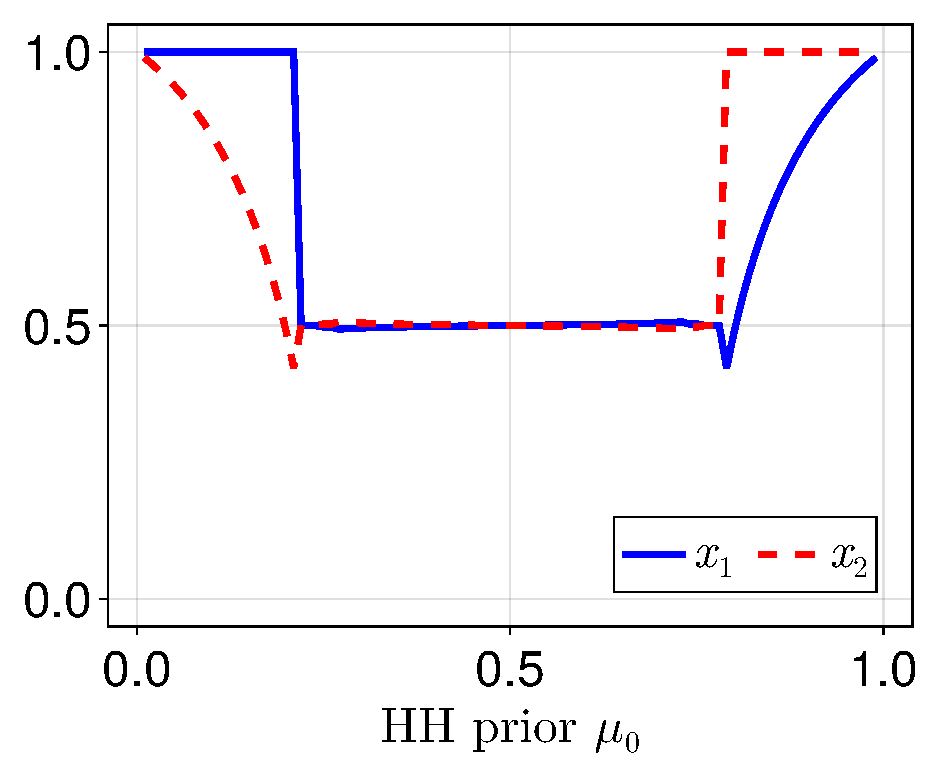
\includegraphics[width=0.49\textwidth]{figures/V8/γ_1/fig_optimal_π_across_μ_0_ω_1_1_ω_2_-1_δ_0.5_.pdf}
    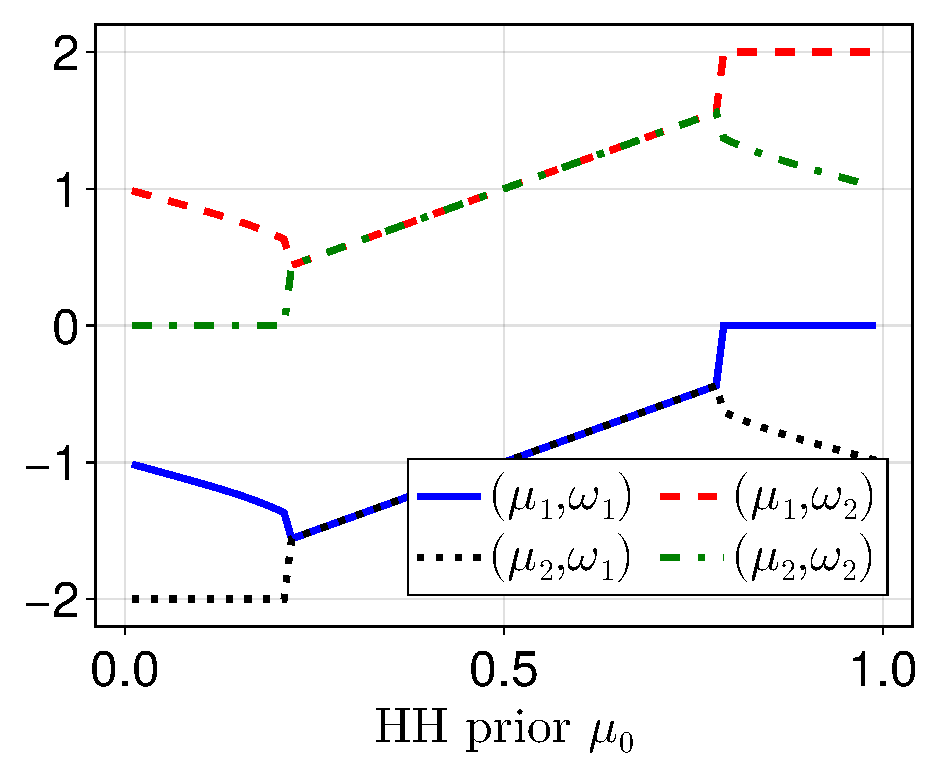
\includegraphics[width=0.49\textwidth]{figures/V8/γ_1/fig_posterior_across_μ_0_ω_1_1_ω_2_-1_δ_0.5_.pdf}
    \end{figure}
    CB responds to excessive optimism or pessimism by HHs inducing the optimal inflation surprise when the shock that HHs consider the least plausible realizes.
    \framebreak
    \begin{figure}[htp!]
    \centering
    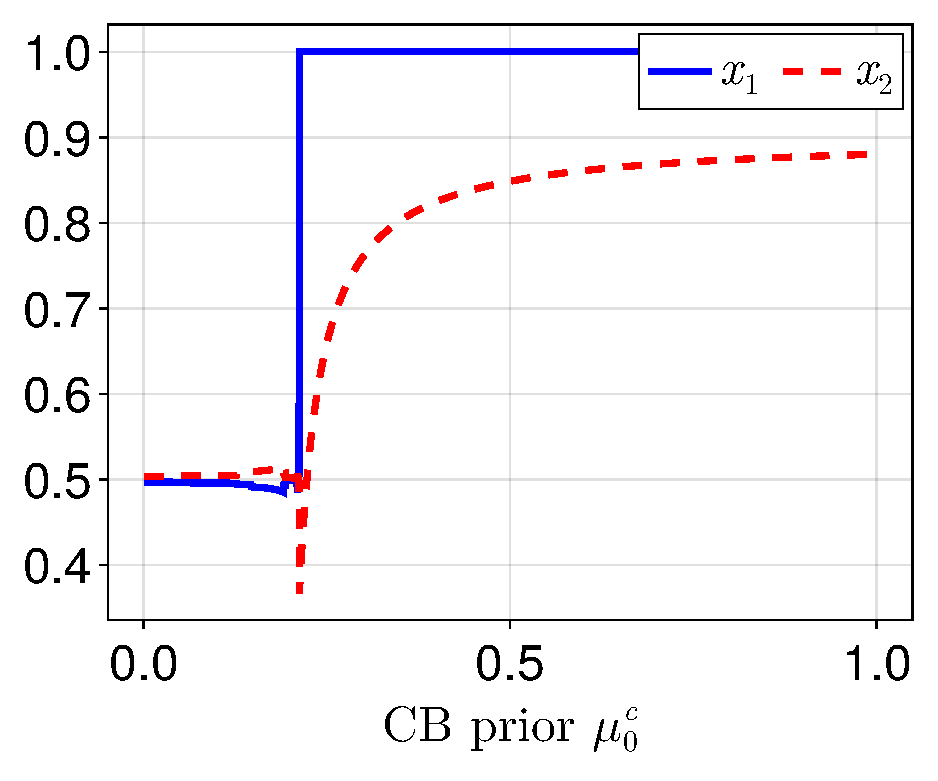
\includegraphics[width=0.49\textwidth]{figures/V9/γ_1/fig_optimal_x_μ_0_c_μ_0_0.1.pdf}
    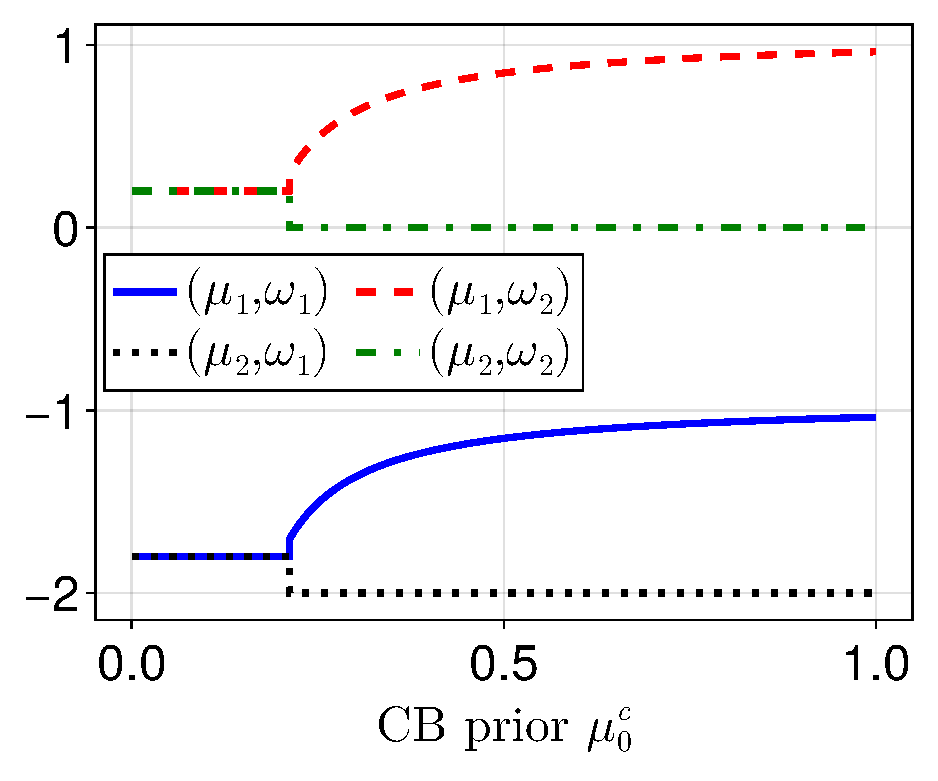
\includegraphics[width=0.49\textwidth]{figures/V9/γ_1/fig_optimal_γ_μ_0_c_μ_0_0.1.pdf}
    \end{figure}
    Assume HHs are optimistic ($\mu_0 = 0.1$). CB intervenes when it does not share such optimism.
    \vskip10pt
    \framebreak
    \begin{figure}[htp!]
    \centering
    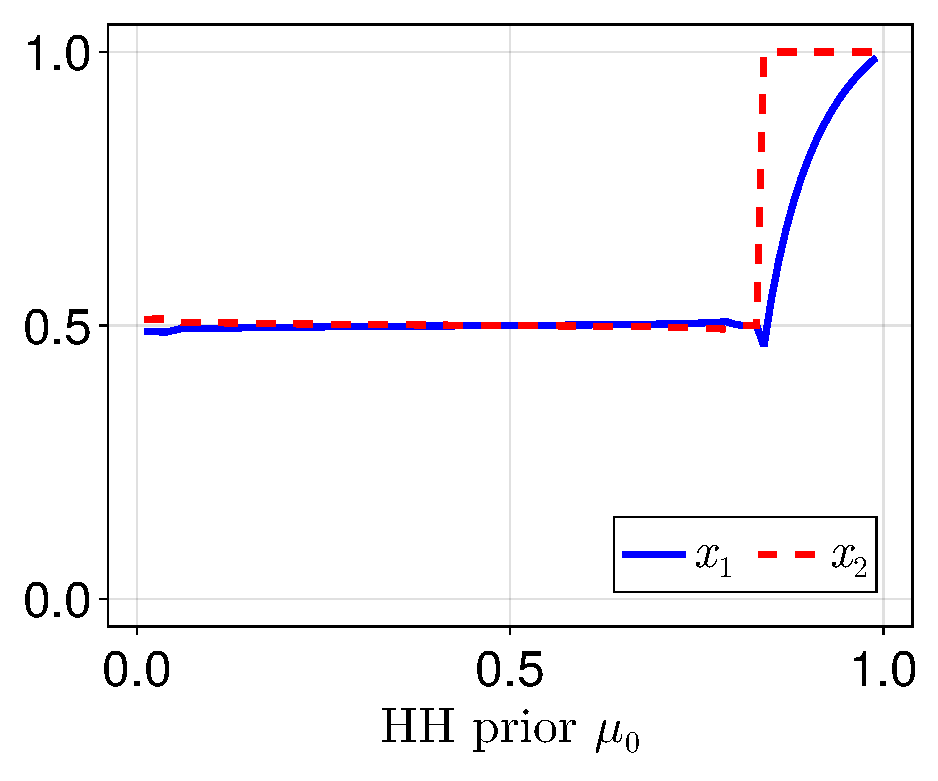
\includegraphics[width=0.49\textwidth]{figures/V8/γ_1/fig_optimal_π_across_μ_0_ω_1_2_ω_2_-1_δ_0.5_.pdf}
    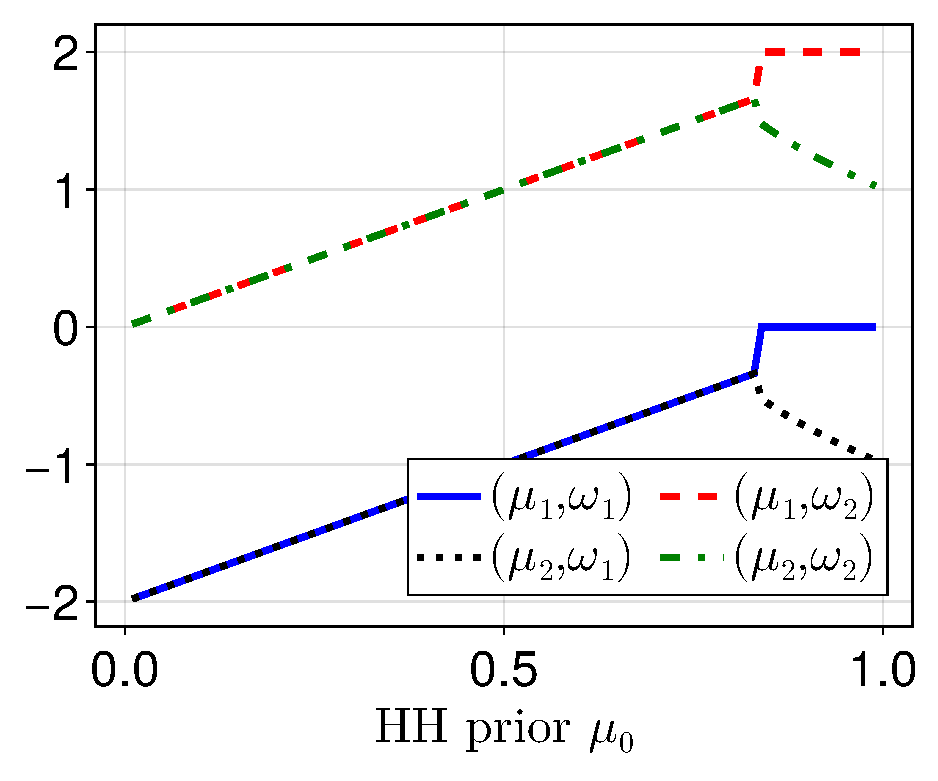
\includegraphics[width=0.49\textwidth]{figures/V8/γ_1/fig_posterior_across_μ_0_ω_1_2_ω_2_-1_δ_0.5_.pdf}
    \end{figure}
    If the bad shock becomes more devastating ($\omega_1=2$), information provision is asymmetric because the inflation surprise is excessive only if HHs are too pessimistic.
    \vskip10pt
    \framebreak
    Now we consider the first stage, endogenizing $\nu_1$ and $\nu_2$.
    \vskip10pt
    We set $\alpha=0$ and all other parameters as before.
    \vskip10pt
    We run comparative statics for the optimal flexibility, and study how this impact the optimal information design.
    \vskip10pt
    \framebreak
    \begin{figure}[H]
    \centering
    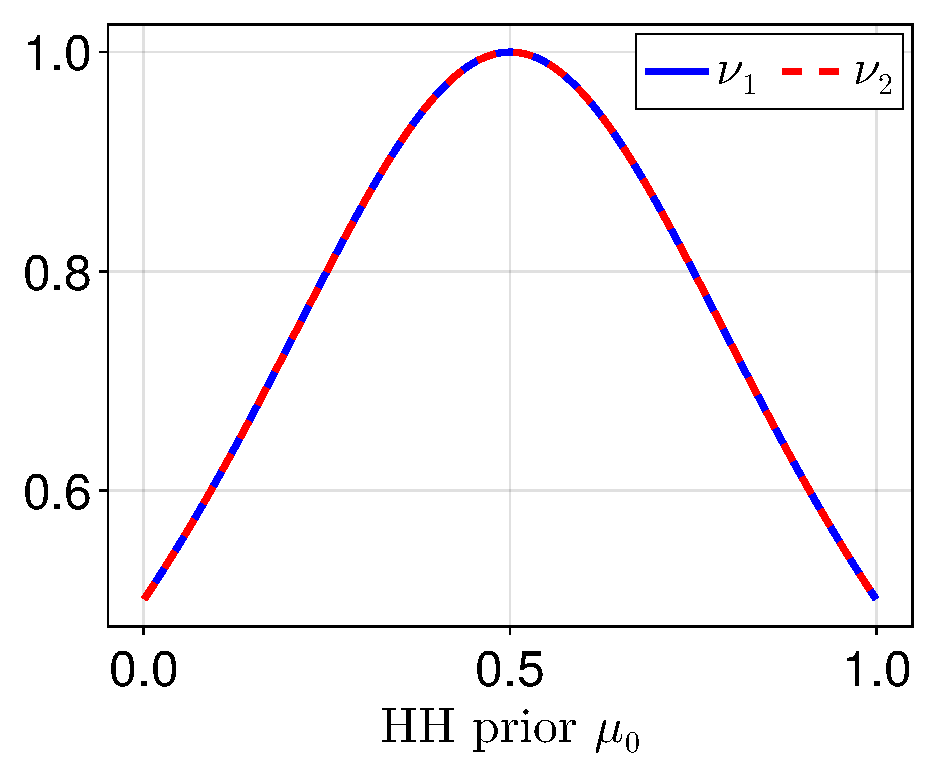
\includegraphics[width=0.49\textwidth]{figures/V9/γ=1.0-μ_0=0.5-α=0.0/fig_optimal_ν_by_μ_0.pdf}
    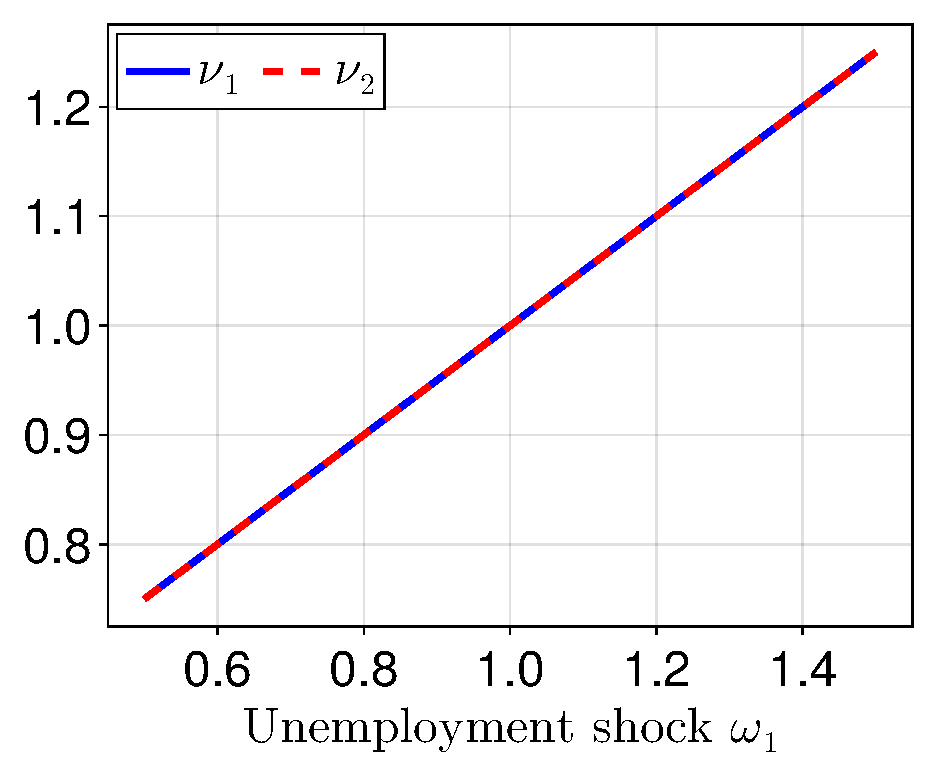
\includegraphics[width=0.49\textwidth]{figures/V9/γ=1.0-μ_0=0.5-α=0.0/fig_optimal_ν_by_ω_1.pdf}
    \end{figure}
    When HHs becomes more certain about the state (in either direction), CB finds it optimal
    to allow for less flexibility.
    \vskip10pt
    Optimal flexibility increases in the total magnitude of the shocks, but it remains symmetric even when shocks are asymmetric.
    \vskip10pt
    \framebreak
    \begin{figure}[H]
    \centering
    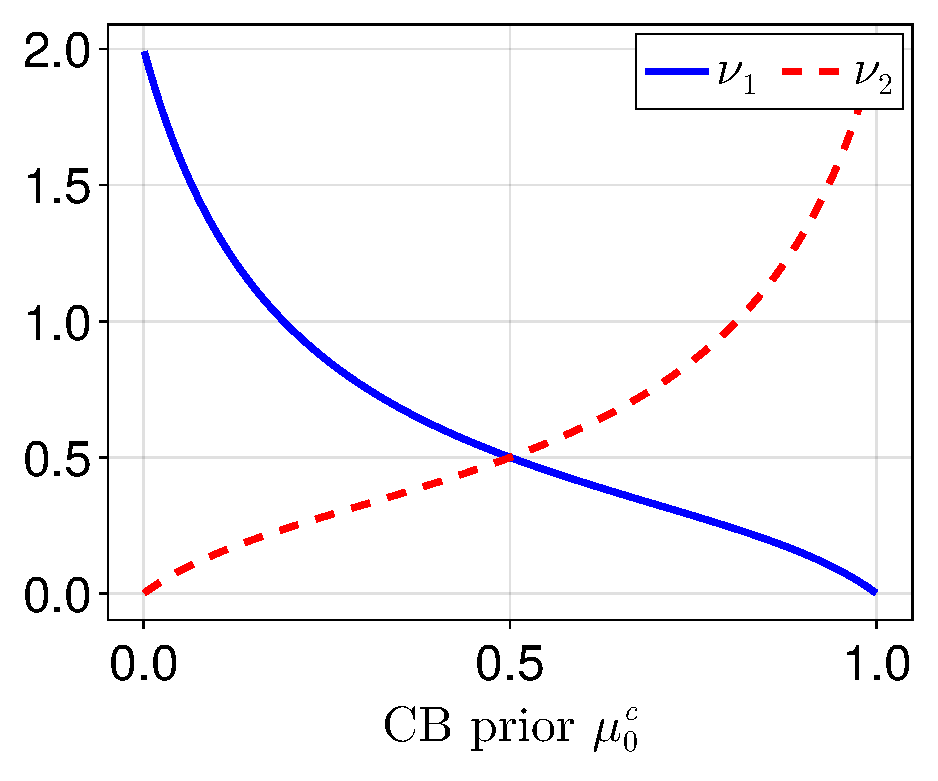
\includegraphics[width=0.48\textwidth]{figures/V9/γ_1/fig_optimal_ν_μ_0_c.pdf}
    \end{figure}
    CB's prior plays a role only when $\alpha>0$ because the induced inflation surprise is insufficient to compensate for shocks.
    \vskip10pt
    Assume $\alpha=1$. When CB is more confident about the nature of the state, CB allows more flexibility in the least likely state, so to reduce the expected inflation gap.
    \vskip10pt
    \framebreak
    When we consider optimal flexibility, the optimal information is always uninformative.
    \vskip10pt
    When $\alpha=0$, optimal flexibility perfectly compensate the shocks.
    \vskip10pt
    When $\alpha>0$, optimal flexibility is lower. However, this corresponds to the case where shocks are relatively large and it is optimal to provide no information.
    \vskip10pt
    Information design is useful only if the monetary policy's flexibility turns out to be excessive ex post.
\end{frame}


\begin{frame}
	\frametitle{Conclusion}
    We find that communication is a tool the central bank uses only if its monetary policy is sub-optimal given the economic fundamentals.
    \vskip10pt
    The central bank provides information if
    \begin{enumerate}
        \item the shock is small and thus the inflation surprise excessive, thus it is optimal to remove uncertainty.
        \item the shock is relatively large but households are either too optimistic or too pessimistic, making the inflation surprise excessive when the state that households consider unlikely realize.
    \end{enumerate}
    \vskip10pt
    We are happy to hear your suggestions!
\end{frame}

\begin{frame}
	\begin{huge}
		\centerline{Thank you for your attention!}
	\end{huge}
\end{frame}

\begin{frame}<presentation:0>[noframenumbering]
	\bibliographystyle{ecta}
	\bibliography{references}
\end{frame}


\end{document}